\chapter{Results}



\section{\Piezo{} as integrator of mechanical shear forces in MSCs}
\label{sec:piezo1-as-integrator-of-biomecshanical-events-in-mscs}

---
In this chapter we want to find out whether piezo1 really also mediates mechanotransduction in MSCs. How do you find something out. So basically what we want to find out is whether Piezo is expressed and functional. What we could do is just staining. Next to mechanosensors being relatively rare in density (GUY from Book Chapter) we would still be missing functionality approval. We know Piezo1 reacts to shear forces (REF) and elicits a measurable calcium influx response. So to functionally proof the contribution of Piezo1 in mechanosensing, we must proof that MSC sense shear, and that they exhibit calcium influx of extracellular calcium and in a second step proof that this does not happen without Piezo
---

In this chapter we want to find out whether \Piezo{} contributes to MSC mechanosensation. Generically speaking, the functional contribution by a component to a certain dynamic can be proven in two steps. We first have to demonstrate an environment where the dynamic is controllably triggered and objectively measurable. Then in a second step by removing the putatively contributing component from the system and by trying to provoke the dynamic again, one can, through the absence of the dynamic, deduce the contribution of the component to the dynamic. In this case, the component is \Piezo{}. Additionally, we know that \Piezo{}, when activated, elicits an influx of extracellular \calcium{}-ions, which describes the dynamic in the generic reasoning. Evidently, we need to establish a platform, where we show that shear forces elicit an influx of extracellular \calcium{}-ions in MSCs. 

For our first experiment, flow chambers were prepared with MSCs being seeded and stained with a calcium-indicator as described in chapter~\vref{sec:LiveImaging}. Then, following the protocol described in the same chapter, we twice in sequence applied a shear pulse and imaged the fluorescent signal, switching the availability of extracellular \calcium{}-ions in between the two measurements. Analysis showed a maximum increase of up to 80\% in fluorescence signal in direct response to shear pulse as opposed to largely absent pulse response in the calcium-free measurement (see Figure \ref{fig:CalcImaging_Cells}a). While the amplitude is likely a function of intracellular state, we oberseve a clear-cut necessity of extracellular calcium-ion presence for intracellular calcium responses. The slight increase in baseline fluorescence in the second  measurement is likely due to the calcium-starved cell replenishing their intracellular calcium-storages after regaining extracellular supply. The negative slope of the baseline is probably due to photobleaching

 

from piezo1 paper we know that PIezo1 makes way for Calcium when activated. With a

Method of choice is shear stress setup described earlier, reference

\begin{figure}
\centering
\includegraphics[width = 0.7\textwidth]{Combined_CalciumFree_KnockOut.png}
\caption{\Piezo{}-mediated influx of extracellular \calciumS confirmed as shear sensing event in MSC. \hfill \newline 
\textbf{a)} Representative fluorescence level measurement of impulse response with two different media where arrows mark the start of a 7Pa shear stress period of 5s. (Pooled data of 4 technical replicates, Data is mean $\pm$ SEM, where area between whiskers is coloured black).	
\textbf{b)} Peak values of fluorescence levels of samples in calcium-free and calcium-containing medium (n = 3, *p $<$ 0.05, Student's t-test with Holm-Sidak multiple correction comparison). 
\textbf{c)} Temporally resolved fluorescence signal of \Piezo{}-KO compared to No-Target cell lines in response to 7 Pa shear period of 5s as denoted by arrow. 
\textbf{d)} Relative amount of cells that showed fluorescence level impulse response. (Data points describe technical replicates, ***p$<$0.0001, ANOVA with Dunnette's multiple comparison test, Data is mean $\pm$ SEM)}
\label{fig:CalcImaging_Cells}
\end{figure}

We demonstrated that MSCs exhibit reactive mechanosensitive capabilities through force-mediated rapid onset influx of extracellular calcium-ions. The role of \Piezo{} in this process, however, is not defined. To examine the contribution of \Piezo{} we compared the impulse response capabilities of two distinct \Piezo{}-knock out constructs to a control cell line.\\
In preparation for this experiment three transfected cell lines were generated (2 distinct \Piezo{} knock-out's and one negative control) using pre-made lentivirus, carrying a CRISPR/Cas9-system with puromycin resistance as the selection marker. The grouping is specified through the Lentiviral Construct used, resulting in cell line P1-395 (meaning the guide-RNA targets the 395\textsuperscript{th} base of \PiezoGene{}), P1-555 and NoT (No Target, Control for the viral treatment with no putative genome mutation). In order to assess knock-out efficiency, both Western Blot and qRT-PCR were done after which we were able to consider this cell line a valid knock-out model (see Fig. \ref{fig:KO-Verification}).\\

\begin{figure}
	\centering
	\includegraphics[width=\linewidth]{Piezo1KO_Verification_WBandPCR.png}
	\caption{Validation of knockout on mRNA (left) and Protein (right) level. P1-395 describes cell line with base deletion in \PiezoGene{}-gene at position 395, similarly P1-555 describes deletion at position 555. NoT describes control for viral treatment with no putative mutation in genome. Protein: n = 1, mRNA:  n$_{P1-395}$ = 2, n\textsubscript{P1-555, NoT} = 3.}
	\label{fig:KO-Verification}
\end{figure}

We then seeded cells in flow chambers and measured the intracellular calcium signal of the cells in response to a shear pulse, similar to the protocol from the previous experiment but only with a single measurement per flow chamber with normal ACSF as shear flow medium. Intriguingly, the \PiezoGene{} knock-out cells show a significantly reduced reaction capability when compared to control (see Figure \ref{fig:CalcImaging_Cells}c,d). When comparing the relative amount of knock-out cells that exhibit calcium-influx in response to shear stress, we see a 66\% decrease compared to control, with the effect being bigger in P1-395 (-73\%) as in P1-555 (-60\%). Interestingly, this difference between two different constructs regarding their reduction of impulse response correlates with the knock-out efficiency. On the lower left plot, we see the same data as in the lower right, but over full temporal resolution and it illustrates how the area under the curve is largely reduced when \Piezo{} is knocked out. 
These results confirm that \Piezo{} is the main driver in force-mediated calcium-influx in mesenchymal stem cells.

\section{\Piezo{} and extracellular matrix production}
\label{sec:PiezoandECM}

Preliminary mass spectroscopy secretome analysis of \Yoda-treated stromal cells showed a distinct decrease in core extracellular matrix (ECM) components, such as alpha-1 type I collagen (\colone), Fibronectin-1 (FN1) and alpha-1 type III collagen (\colthree) (Not shown here, personal communication with Fabian Passini and Ulrich Blache). This led to further investigation into this matter.\par

After seeding cells in serum-free medium and letting them rest, we chemically stimulated \Piezo{} with \Yoda{} during 30 minutes, before washing them and transferring them in the incubator again, following the protocol described earlier in section ~\vref{sec:ChemicalStimulation}. We then harvested control samples right after intervention (denoted by d0) and \Yoda{}- and control samples after 24, 48 and 72 hours (d1, d2 and d3, respectively) to achieve temporal resolution. \par

\begin{figure}[htbp]
	\centering
	\includegraphics[width = 0.9\textwidth]{NormalYodaExp_WesternBlot_Col1a1.png}
	\caption{ Western Blot analysis of intracellular protein in \Yoda{}-treated MSCs over time (d1: 24h, d2: 48h, d3: 72h) compared to \Yoda{}-control samples harvested at the same time.
		\textbf{a.)} Representative Chemiluminescence for \colone with control and chemically stimulated \Piezo{}-samples with alpha-Tubulin as housekeeper.
		\textbf{b.)} Quantification of repeated experiments, each data point normalized against housekeeping protein (loading correction) and corresponding d1, control-sample (donor-specific correction) (Student's t-test with Holm-Sidak multiple comparison correction, Data is mean $\pm$ SD, Amount of protein loaded varies between \myworries{WHAT})}
	\label{fig:Yoda_Norm_WB}
\end{figure}


\begin{figure}
	\centering
	\includegraphics[width=0.7\linewidth]{Uli_Blot_KO.png}
	\caption{Western Blot of selected ECM components comparing protein content of different MSC lines 3 days after 30min exposure to either MEM\textalpha{} only (negative control) or MEM\textalpha{} supplemented with 5\textmu{}M chemical \Piezo{} agonist (YODA +), \textalpha{}-Tubulin as housekeeping protein.}
	\label{pic:UliBlot}
\end{figure}

Western Blot Analysis of intracellular protein showed a trend of declining \colone-content in samples that have been treated with \Yoda{} (As shown in \ref{fig:Yoda_Norm_WB}). Furthermore, the effects were not only marked by fast onset but also of long-lasting nature, since the effect of a singular 30 minutes \Yoda{}-exposition remained the same three days after intervention. There were inconsistencies in our housekeeping protein bands, indicating possible loading problems. Similar effects can also be seen in \textsc{Fn1} and \colthree{} (see Figure~\vref{pic:UliBlot}.) \par

Using qRT-PCR, we also looked at mRNA representation while focusing on \coloneGene{}, \colthreeGene{}, \Fn{} and \textit{Interleukin-6} (\ILGene{}) with \textit{GAPDH} and \textit{RPL13A} as house-keeping genes. All measurements were normalised against negative control samples harvested immediately after the intervention. \\
\ILGene results are not significant, due to high variance. However, there is a trend of a sharp increase in \Yoda{} samples from d0 to d1 followed by a relaxation over following three days to original levels. This tendency is interesting, but it remains to be investigated, whether it translates to a \textit{de facto} increase in bioactive \IL protein. mRNA levels of \colone{} show a decreasing trend over time, while \colthree and \textsc{Fn}1 stayed largely the same (see Fig. \ref{fig:Yoda_Norm_PCR})\par

\begin{figure}[ht]
	\centering
	\includegraphics[width = 0.7\textwidth]{NormalYodaExp_PCR.png}
	\caption{mRNA levels of selected gene products in naive MSCs after 30min chemical stimulation of \Piezo{}, harvested after 24, 48 or 72 hours (denoted by d1, d2 or d3, respectively). Normalized against d0, control.
	    \textbf{a.)}: \coloneGene{}
		\textbf{b.)}: \ILGene{}
		\textbf{c.)}: \colthreeGene{}
		\textbf{d.)}: \FnGene, 
		(Student's t-test with HSmcc, n = 4, Data is mean $\pm$ SD). 
	}
	\label{fig:Yoda_Norm_PCR}
\end{figure}




\section{Reversibility and osteogenic differentiation of \Yoda{}-treated cells}

\begin{figure}[ht]
	\centering
	\includegraphics[width = \linewidth{}]{LongTerm_CellPicture.png}
	\caption{
		Light microscopy picture taken of cells seven days after intervention with either 0\textmu{}M (Yoda: -) or 5\textmu{}M (Yoda: +) chemical \Piezo{}-agonist. Three days after intervention, medium was replaced with either serum-free MEM\textalpha{} (Serum: -) or MEM\textalpha{} supplemented with 10\% FBS (Serum +).}
	\label{pic:Cells_LongTerm}
\end{figure}

\begin{figure}
	\centering
	\includegraphics[width = \linewidth{}]{LongTerm_PCR.png}
	\caption{RNA level analysis of different genes in MSCs seven days after exposure to chemical \Piezo{}-agonist, following a modified version of the protocol described in chapter~\ref{sec:ChemicalStimulation}. Each sample is normalized against respective \Piezo{}-agonist control samples. We changed the media three days after intervention and supplemented MEM\textalpha{} with either 0\% (Serum -) or 10\% FBS (Serum: +) (n = 1).}
	\label{fig:LongTerm_PCR}
\end{figure}

Because we found that intracellular \colone{} protein levels did not recover during our previously chosen time frame, we wanted to investigate whether the \Yoda{}-treated cells would reach a pre-intervention state after a longer duration. For this reason, we decided to repeat the experiment from before, but only harvesting the cells after seven days. Because in the experiment before we saw a change in cell morphology in \Yoda{}-treated samples, which indicates a decrease in cell viability (see Fig. \ref{pic:Yoda_Apop}), we adapted the protocol to ensure cell viability. The medium was changed three days after the intervention, where one group of cells received serum-free MEM\textalpha{} (S-), whereas the other half was administered MEM\textalpha{} with 10\% FBS (S+). For this experiment we only did qRT-PCR, due to very low yield in the serum-starved \Yoda{}-group (S-\textbackslash{}Y+)). All samples were pooled triplicates and normalized against negative \Yoda{}-control samples from day 7.\\
Interestingly, in our experiment the RNA levels of \colone{} were still drastically lowered independent from FBS supplementation, with as low as 12\% in the serum-starved group. While \colthreeGene{} was also low, this could also be explained by a great variance, which we saw in the experiment before (see Fig. \ref{fig:Yoda_Norm_PCR}). \ILGene{} and \FnGene{} was slightly reduced. It is important to keep in mind, due to the experiment being a single measurement, this qualifies only as an exploratory experiment at best. However, there are some plausible indications. For example, it is interesting to note, that \ILGene{} seemed to recover completely to pre-intervention level, as implied in the experiment before. \\
Furthermore, when looking at \coloneGene{} in serum-supplemented \Yoda{}-samples, while the PCR levels remained low (see Fig.~\vref{fig:LongTerm_PCR}), the cells exhibited a spindle-like morphology and regained proliferative capacity, as opposed to the rounded and sparsely distributed cells observed in serum-starved samples (see Fig.~\ref{pic:Cells_LongTerm}). This implies that \Piezo{}-mediated downregulation of ECM components and decrease of cell viability are mediated by two independent pathways, both downstream of \Piezo{}, as the decrease in cell viability discussed in the next chapter seems neutralised by addition of FBS, whereas the downregulation of \coloneGene{} seemingly is not.\\
One alternative explanation would be that the applied \Yoda{}-stimulus leads to a persistent change and possibly to differentiation.\par

Sugimoto and colleagues suggested that \Piezo{} activation leads to osteogenic differentiation \cite{Sugimoto2017}. To test whether we reproduced their results by \Piezo{}-activation, we employed the same protocol, consisting of 30min 5\textmu{}M \Yoda{} exposure with the only experimental sample from day 3, which then are normalised against negative control samples harvested right after the intervention. As read-out method we chose qRT-PCR, following Sugimoto's paper, and focused our analysis against both early osteogenic genes like RUNX2 and late osteogenic genes like ALPL and SPP1 \cite{Creecy2013, Marom2005}. \par


\begin{figure}[htbp]
	\centering
	\includegraphics[width = \linewidth]{Osteogenic_PCR_Yoda.png}
	\caption{mRNA transcript levels of different late and early osteogenic markers, comparing MSCs 3 days after \Yoda{}-intervention (30min of 5\mul{}M \Yoda{} in MEM\textalpha{}) to \Yoda{} control (only MEM\textalpha{}) and normalised against \Yoda{} control samples, harvested directly after intervention ended (n=3, Student's t-test with Holm-Sidak multiple comparison correction).}
	\label{fig:Osteo_PCR}
\end{figure}
 

Our results showed no significant differences. However, this does not mean, that we can exclude \Piezo{} implicated in osteogenic differentiation. One central aspect of Sugimoto's study was the existence of a certain "sweet-spot" of hydrostatic pressure where osteogenic differentiation happens, after which increasing pressure would lead to insignificant results. It is plausible that the quality our \Piezo{} stimulus would need adaptation for successful reproduction of Sugimoto's results.



\section{Biostability of \Yoda{} and \Piezo{} mediated decrease in cell viability}
\label{sec:biostability}


\begin{figure}[h!]
	\centering
	\includegraphics[width = 0.85\linewidth]{Yoda_Apoptosis.png}
	\caption{Light microscopy picture of serum-starved cells 7 days after intervention with 0\textmu{}M (Control) or 5\textmu{}M (Yoda) chemical \Piezo{}-agonist.}
	\label{pic:Yoda_Apop}
\end{figure}

We realised there was a continuous decrease in cell count in \Yoda{}-treated cells (see Fig.~\ref{pic:Yoda_Apop}). Next to \Piezo{} being implicated in this decrease in cell viability, an intrinsic cytotoxicity of \Yoda{} could also be an explanation. To test this hypothesis, Dr. Ulrich Blache exposed, in an explorative experiment, both \Piezo{}-KO and NoT cell lines to \Yoda{}, using a protocol similar to the one described in chapter ~\vref{sec:ChemicalStimulation}. The results of this experiment suggestested that the effect was \Piezo{} dependent (not shown). Further experiments are needed to make any conclusions. However, this observation could be explained with calpain activation, downstream of \Piezo{}, that has known pro-apoptotic effects through caspase-3 and caspase-12 activation \cite{Altznauer2004, Nakagawa2000}. Furthermore, there is evidence that relates different intracellular calcium concentration to a set of cellular mechanisms, including apoptosis. Here it might be worthwhile, to alter experimental \Yoda{} concentration to explore different regions of the continuous cellular process spectrum. Another thing to keep in mind is that \Yoda{} activity might not only vary with concentration but also with time.

\begin{figure}
	\centering
	\includegraphics[width = 0.4\linewidth{}]{Inkubationshypothese.png}
	\caption{Intracellular protein analysis of MSCs one day after undergoing a modified version of the protocol described in chapter~\ref{sec:ChemicalStimulation}. We altered both the concentration of \Piezo{}-agonist \Yoda{} in intervention medium and duration of \Yoda{} incubation before being added to the cells. For all groups, the respective intervention medium was pre-incubated for 8 hours at standard incubation conditions. One intervention medium was pre-incubated with 5 \textmu{}M \Yoda{} (8h Yoda Intervention), another intervention medium was supplemented with 5 \textmu{}M \Yoda{} only after pre-incubation, right before giving it to the cells (No Yoda Intervention) and third group was \Yoda{} control (Control).}
	\label{fig:Inkubationshypothese_Western}
\end{figure}

Our observations suggested that in standard incubation conditions \Yoda{} is transformed and loses its effect over time (not shown). To test this hypothesis, we employed a modified version of the protocol described in chapter~\ref{sec:ChemicalStimulation}. We altered both the amount of \Yoda{} in the intervention medium and duration of \Yoda{} pre-incubation before being added to the cells. For all groups, we introduced a pre-incubation period of 8 hours, durng which the respective intervention medium was incubated at standard incubation conditions. One intervention medium was incubated containing 5 \mul{}M \Yoda{} (8h Yoda Invervention), another intervention medium was supplemented with 5 \mul{}M \Yoda{} only after pre-incubation, right before giving it to the cells (No Yoda Intervention) and third group was \Yoda{} control (Control). We found that incubation of \Yoda{} during a certain amount of time seems to diminish its bioactivity completely (see Fig.~\ref{fig:Inkubationshypothese_Western}). This has not been published knowledge, but should be considered in future study designs.

\chapter{Discussion}



PROTEIN DISCUSSION:


Interestingly, the trend of \colone{}, \colthree{} and \Fn{} being largely reduced on protein level is not reflected by the mRNA representation. Since mRNA levels are unchanged and secretome analysis reflects the decrease seen in intracellular protein, the effect of the intervention likely acts between transcription of mRNA and secretion of the protein. \\


ECM components are known to be post-transcriptionally modified both in the endoplasmatic reticulum (ER) and in the endosomes, which are the transporter entities involved in the secretion \cite{Ishida2011, Zeltz2014}. This makes additional studies necessary for more sophisticated hypothesis. One possible explanation for the observation could be calpain, a protease that relies on calcium as a cofactor for effector function \cite{Goll2003}. McHugh and colleagues produced evidence for calpain being a downstream effector of \Piezo{} \cite{McHugh2010}. Furthermore, there are studies that link calpain activity to skin wound healing, which is heavily dependent on ECM and specifically \colone{} \cite{Nassar2012}. However, in this paper, Nassar and colleagues demonstrate that calpain-inhibition leads to reduction of \colone{} mRNA, which implicitly contradicts our data. To further investigate this dynamic, it might be worthwhile to investigate the relationship between \Piezo{}-dependent calcium influx and subsequent activation of calpain. \par

Important to note is that cells were previously cultured with 5 \textmu{}g/ml FGF-2 and 10\% FBS, before they were serum-starved and FGF-2 deprived for the experiment. This likely leads to confounding factor including differentiation, which would have to be addressed in future studies.\par

In conclusion, this divergence between decreased protein with largely normal mRNA levels as a consequence of \Piezo{} stimulation introduces a new dimension, inspiring further research into the topic.
